\documentclass[11pt,a4paper]{article}
\usepackage[utf8]{inputenc}
\usepackage[T1]{fontenc}
\usepackage[francais]{babel}
%\usepackage{fullpage}
\usepackage{gensymb}
\usepackage{graphicx}
\usepackage{float}
\usepackage{amsmath}

\begin{document}

Page de garde

\newpage

\section{Présentation du projet}

\subsection{Objectif général}
L'objectif général de notre projet de fin d'études, dit \textit{PFE}, est d'étudier et de mettre en place une chaîne de transmission vidéo.
Nous ferons une étude technique et la réalisation de l'ensemble des étapes : de la station émettrice au récepteur, en passant par les techniques de mise en réseau.

\bigbreak
Nous avons décidé de nous intéresser plus particulièrement à l'amélioration de la qualité d'une zone géographique d'un flux vidéo, au détriment du reste de la vidéo.

Ce principe peut se révéler intéressant dans des cas où le consommateur d'un flux vidéo ne serait intéressé que par une zone précise d'une image capturée par une caméra, tout en étant susceptible de changer de zone d'intérêt à tout instant.
La zone d'intérêt est choisie et commandée par le client récepteur du flux vidéo, afin que l'émetteur puisse adapter la zone d’intérêt pour la suite de la transmission.

\bigbreak
Nous essaierons de faire des choix technologiques les plus simples et compréhensibles possibles et d'assurer une interopérabilité entre différentes plateformes matérielles et logicielles.

\subsection{Cas d'application}

Afin d'illustrer ce système en pratique, nous l'implémenterons au sein d'une solution de transmission vidéo distante en réalité virtuelle.
Une station émettrice mobile capture un flux vidéo provenant d'une caméra à grand angle et transmet un flux qui sera alors reçu sur un autre terminal mobile n'affichant qu'une zone précise de l'image à travers une solution de réalité virtuelle de type Google Cardboard.
Le terminal est donc déplacé avec les mouvements de tête du spectateur et la zone de visionnage est donc déplacée en conséquence pour obtenir un effet immersif.
La nouvelle région d’intérêt est renvoyée du terminal mobile à l'émetteur pour faire à nouveau coïncider la zone visionnée avec la région d'intérêt à qualité améliorée.

\subsection{Contraintes qualitatives}

Nous avons la contrainte de transmettre l’ensemble de la vidéo pour pouvoir répondre instantanément aux déplacements de la tête de spectateur.
En effet, des solutions existantes comme celle choisie par certains drones tels que celui de Parrot font le choix de ne transmettre que la région d’intérêt. Cela présente l’inconvénient de devoir attendre un aller/retour complet de transmission avant d’avoir l’image demandée. Pour un effet immersif complet, cela ne peut pas être envisagé.
D’autres solutions font le choix de simplement transmettre l’image complète non-modifiée, assurant ainsi une image de qualité moyenne sur l’ensemble de la scène.

\bigbreak
Notre solution devra donc permettre d’avoir une qualité supérieure de la zone observée au prix d’une dégradation du reste de l’image.
Ainsi, lorsque le spectateur bouge la tête, il voit immédiatement la partie de l’image correspondante, mais en qualité dégradée. Il faudra attendre l’aller/retour complet pour obtenir une image de bonne qualité.

\bigbreak
Pour pouvoir mesurer une amélioration de la qualité et s’adapter à diverses conditions de transmissions réseau, nous utiliserons un encodeur à débit contraint, de telle sorte que ce soit la qualité qui soit variable.
Ce débit pourra d’ailleurs être adapté en fonction des pertes réseaux observées par le récepteur.


\section{Recherche}

Nous avons sélectionné quelques papiers qui s'intéressent à des techniques s'approchant de notre projet : la compression vidéo avec une qualité variable en fonction de la zone d'intérêt de l'utilisateur.

\bigbreak
La solution la plus évidente est d'intervenir directement au niveau de l'algorithme de compression.
L'article de Amir Said et William Pearlman\ref{REF1} décrit comment compresser une image avec un débit variable pour chaque partie de l'image.

Cette approche est intéressante mais nous faisons le choix de réutiliser un algorithme de compression, dit \textit{codec}, existant.
L'algorithme étant notamment déjà intégré dans les terminaux de réception pour effectuer du décodage matériel, il nous est presque impossible d'intervenir à ce niveau.

\bigbreak
L'article de Engin Kurutepe\ref{REF2} montre comment optimiser l'envoi d'un flux provenant de plusieurs caméras.
Pour cela, l'équipement récepteur suit les mouvements de la tête de l'utilisateur afin de savoir quelle zone de l'image l'intéresse le plus.
Après cela, l'équipement envoie cette information à l'encodageur qui va demander un plus gros débit aux caméras qui filment la zone d'intérêt et un débit plus faible aux autres caméras.

Nous ne pouvons pas réutiliser ce concept car nous n'avons qu'une seule caméra qui filme la scène et le principe décrit par l'article est applicable seulement pour une même scène filmée avec plusieurs caméras.
Cela nous a tout de même confortés dans l'idée d'encoder une vidéo sphérique avec une qualité dynamique, mais à l'intérieur d'une même image.

\bigbreak
Enfin, l'article de Aditya Mavlankar et Bernd Girod\ref{REF3} explique comment optimiser l’envoi d’une image basse qualité d’un match de football ainsi qu’une zone précise de haute qualité.
L’idée ressemble à ce que nous voulons faire, mais les recherches se portent sur l’optimisation de l’encodage pour du broadcast ; comment éviter d’encoder le flux de haute qualité pour chaque téléspectateur.
Or, notre projet fonctionne dans un modèle mono-utilisateur, il sera donc plus simple et plus efficace pour notre modèle d’encoder le flux entier en prenant directement en compte la zone d'intérêt de l'utilisateur.
Aussi, cet article cite les mécanismes FMO et ASO du standard de compression vidéo H.264 qui permettent respectivement d’avoir un débit différent pour chaque bloc de l'image et de prioriser la qualité des zones de l’image.
Malheureusement, ces plugins ne sont pas implémentés par défaut dans des outils libres comme FFmpeg ou la libx264 et peu de récepteurs mobiles ne les comprennent.

\bigbreak
Globalement, nous n'avons pas pu trouver d'articles décrivant un procédé permettant d'implémenter directement notre projet, nous partirons donc sur l'étude et la conception d'une solution propre.
Cette recherche nous aura tout de même permis d'avoir un bon aperçu des techniques de compression vidéo couramment utilisées.


\section{Architecture générale}

\section{Détails d'implémentation}

\subsection{Acquisition d'image RAW}
Pour notre projet, nous nous sommes procurés une caméra à grand angle (180\degree) pour être en mesure de filmer l'intégralité d'une scène.
\bigbreak
-> Photo Caméra
\bigbreak
La caméra est compatible avec le driver générique \textit{uvcvideo} inclus par défaut dans le noyau Linux, et peut donc être utilisée à travers \textit{Video4Linux 2}, V4L2.

\bigbreak
Afin d'obtenir l'image la moins altérée possible et de faciliter les futurs traitements sur l'image, nous récupérons les images RAW non-compressées.
La caméra est capable, à travers l'USB2, de tenir un flux de données correspondant à des images d'une résolution de 1280x720 à une fréquence de 10 images par seconde.
% Détail sur le débit en sortie du port USB ?

\bigbreak
L'acquisition est réalisée grâce à notre première instance de FFmpeg et à son module d'acquisition V4L2 qui permettent d'obtenir les octets correspondants sur la sortie standard pour la suite de notre traitement.

\bigbreak
La caméra utilisée présente une particularité : le capteur CMOS utilisé est un capteur standard et l'effet grand angle est obtenu par l'apposition d'une lentille convexe au-dessus.
Si cela permet alors d'obtenir un champ de vision très proche de 180\degree, l'image en retour présente un effet \textit{fisheye} non-négligeable.

\bigbreak
-> Capture effet fisheye brut
\bigbreak

Pour rendre des proportions réalistes aux abords de l'image, il est nécessaire de procéder à une correction de la déformation induite par la lentille.
Heureusement, FFmpeg dispose d'un certain nombre de plugins de traitement d'image que nous pouvons utiliser pendant la phase d'acquisition d'image RAW.

\bigbreak
L'un d'entre eux, issu de la collection de plugins \textit{Frei0r}, est le plugin \textit{Defish0r}, relativement simple d'utilisation et qui permet d'annuler cet effet de distorsion.
Malheureusement, les premiers tests ont montré que le plugin était trop gourmand en calcul CPU, et qu'il était impossible de traiter 10 images par seconde : le retard s'accumule rapidement.

\bigbreak
Un autre plugin, plus générique, est présent dans FFmpeg : \textit{lenscorrection}.
Plus léger en calcul, il est capable de traiter nos 10 images par seconde avec notre carte Raspberry Pi 3.
Son inconvénient est son paramétrage : le filtre demande deux coefficient correspondant aux termes de second et quatrième degrés dans la formule de correction :

$$r_{src} = r_{targ} * (1 + k1*(\frac{r_{targ}}{r_0})^2 + k2*(\frac{r_{targ}}{r_0})^4)$$
avec :
\begin{itemize}
\item{$k1$, $k2$ : coefficients considérés}
\item{$r_0$ : moitié de la diagonale de l'image}
\item{$r_{src}$ : distance entre le point considéré dans l'image source et le centre de l'image}
\item{$r_{targ}$ : distance du point à placer dans l'image de destination avec le centre de l'image}
\end{itemize}

\bigbreak

La difficulté réside donc dans la détermination des coefficients $k1$ et $k2$ adaptés à notre configuration capteur+lentille.
Les valeurs se situant dans l'intervalle $[-1;1]$, nous réalisons un test visuel en générant des images avec tous les couples de $(k1, k2)$ possibles en prenant un pas de $p=0.1$, soit une série de 441 images.

\bigbreak
-> Mosaique images ?

\bigbreak
Le détermination des coefficients s'est donc faite de façon qualitative en visionnant la série d'images et en choisissant l'image présentant le moins de déformation tout en évitant les aberrations.
Les valeurs suivantes semblent correspondre à notre lentille :
$$k1 = -0.4, k2 = 0.1$$

\subsection{Traitement de l'image YUV}
Si nous avons maintenant une image brute corrigée, nous souhaitons lui appliquer notre traitement spécifique.

\subsubsection{Format \texttt{YUV 4:2:0}}
L'image RAW d'entrée est donc d'une résolution de 1280x720 avec un codage des pixels selon le format \texttt{YUV 4:2:0}.
Ce format est très utilisé dans le codage de la vidéo car il est adapté à un visionnage par un œil humain : contrairement au format RGB qui code de façon égale les composantes rouge, verte et bleue de la vidéo, le format YUV code une information de luminance et une information de chrominance.
Dans le cas du format \texttt{YUV 4:2:0}, il y a deux fois plus d'informations de luminance que de chrominance, tout simplement car l'œil humain est plus sensible aux différences de luminosité qu'aux différences de teinte.

\bigbreak
Plus précisément, les pixels sont répartis en blocs de 4 pixels (2x2).
Chaque bloc contient 4 informations de luminance (une valeur \texttt{Y} pour chacun des 4 pixels), mais seulement une information de chrominance commune à l'ensemble du bloc (une valeur \texttt{U} et une valeur \texttt{V}).

\begin{figure}[H]
\begin{center}
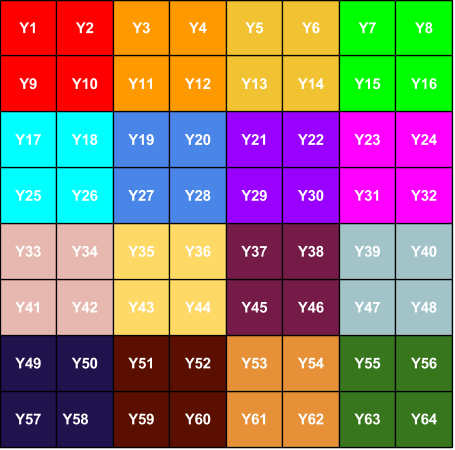
\includegraphics[scale=0.5]{images/yuv1.png}
\end{center}
\caption{Organisation des pixels au sein d'une image \texttt{YUV 4:2:0}}
\label{}
\end{figure}

\bigbreak
Chaque valeur de \texttt{Y}, \texttt{U} et \texttt{V} est codée sur un octet.
Ainsi, la taille d'une image YUV d'une résolution de \texttt{8x8} pixels (16 blocs) peut être calculée comme ceci :

$$ T = 16 * (4Y + 1U + 1V) = \mathbf{96}$$

D'une manière générale, la taille d'une image \texttt{YUV 4:2:0} peut donc se calculer comme étant le nombre de pixels multiplié par $\frac{3}{2}$.
Ainsi, chacune de nos images \texttt{1280x720} a une taille d'environ 1,4 Mo.

\bigbreak
La répartition de ces informations dans la suite d'octets est un peu particulière : on trouve d'abord toutes les valeurs de Y, puis toutes les valeurs U et enfin de V.
La lecture d'un bloc se fait donc en trois lectures consécutives.

\begin{figure}[H]
\begin{center}
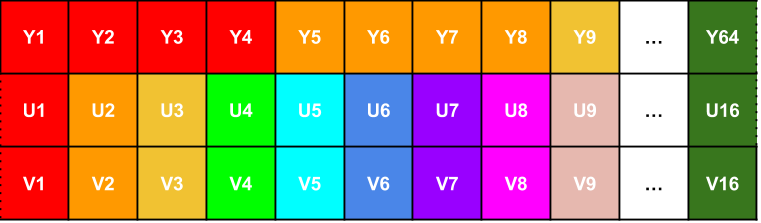
\includegraphics[scale=0.5]{images/yuv2.png}
\end{center}
\caption{Séquence d'information du format \texttt{YUV 4:2:0}}
\label{}
\end{figure}

\bigbreak

\subsubsection{Traitement spécifique}
Puisque nous avons fait le choix de ne pas intervenir au niveau du codec lui-même, nous appliquons un traitement spécifique permettant de sous-échantillonner les zones autres que la zone d'intérêt.
L'idée est de conserver la zone d'intérêt dans sa résolution originelle et de diviser par un facteur quatre les dimensions des autres parties de l'image, c'est-à-dire diviser la largeur et la hauteur par deux.

\bigbreak
La zone d'intérêt a une dimension fixe choisie comme une moitié de largeur et hauteur totales, soit une résolution de \texttt{640x360} ou $\frac{1}{4}$ de la surface de l'image source.
Ainsi, dans l'idéal, notre image traîtée finale a une résolution d'une fraction de celle de l'image source :

$$ R = \frac{1}{4} + \frac{3}{4}*\frac{1}{4} = \mathbf{\frac{7}{16}} $$

Ce résultat est le résultat que nous pourrions obtenir en découpant de façon idéale les zones.
Pour des raisons de complexité de calculs, nous essaierons de garder les zones entières lors de nos déplacements.

\begin{figure}[H]
\begin{center}
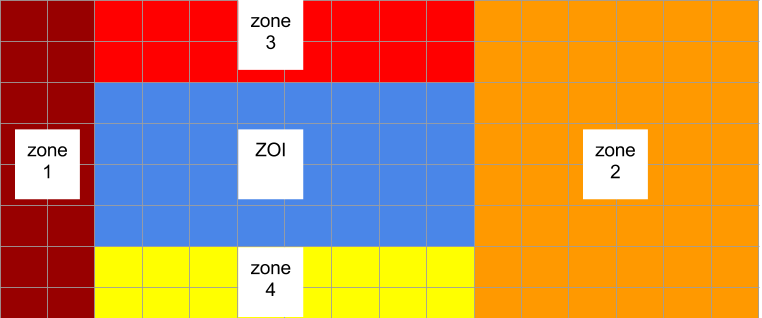
\includegraphics[scale=0.4]{images/decoupage.png}
\end{center}
\caption{Découpage en zones d'une image 16:9}
\label{}
\end{figure}

\bigbreak
La zone d'intérêt, ou ZOI, conserve ses dimensions d'origine : \texttt{640x360}.
Elle est placée dans la seconde moitié de l'image, laissant ainsi une autre fenêtre de \texttt{640x360} pixels libre.

\bigbreak
Pour rappel, la ZOI a une taille fixe mais sa position de départ est variable et contrôlée par le client récepteur.
Ainsi, les autres zones autour de cette ZOI sont de taille variable, en fonction du point de départ de la ZOI qui nous définirons par le couple \texttt{(zoiX, zoiY)}.
Les positions et dimensions des différentes sont alors définies comme cela :
\bigbreak
\begin{itemize}
\item{Zone 1 : position=\texttt{(0, 0)} ; dimensions=\texttt{(zoiX, imgHeight)}}
\item{Zone 2 : position=\texttt{(zoiX+zoiW, 0)} ; dimensions=\texttt{(imgWidth-(zoiX+zoiW), 720)}}
\item{Zone 3 : position=\texttt{(zoiX, 0)} ; dimensions=\texttt{(zoiW, zoiY)}}
\item{Zone 4 : position=\texttt{(zoiX, zoiY+zoiH)} ; dimensions=\texttt{(zoiW, imgHeight-(zoiY+zoiH))}}
\end{itemize}

\bigbreak
avec :
\begin{itemize}
\item{\texttt{(zoiX, zoiY)} : position actuelle de la ZOI}
\item{\texttt{(zoiW, zoiH)} : taille de la ZOI, dans notre cas \texttt{(640, 360)}}
\item{\texttt{imgWidth, imgHeight} : dimensions de l'image d'origine, dans notre cas \texttt{(1280, 720)}}
\end{itemize}

\bigbreak
Les quatre zones sont ensuite sous-échantillonnées : les largeurs et hauteurs sont divisées par deux, procédant ainsi à une réduction de la résolution d'un facteur 4.
Pour cela, nous transformons chaque groupe de quatre blocs YUV en un seul bloc selon le procédé suivant :

\begin{figure}[H]
\begin{center}
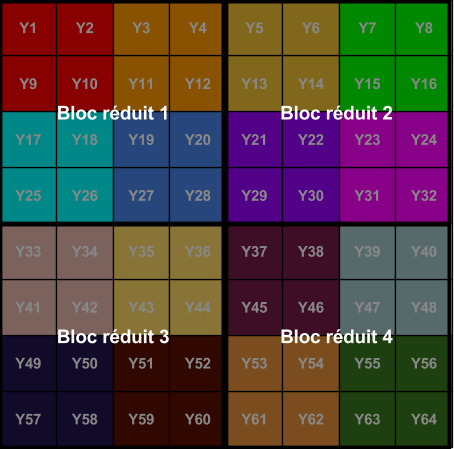
\includegraphics[scale=0.5]{images/yuv3.png}
\end{center}
\caption{Approximation des blocs}
\label{}
\end{figure}

\bigbreak

Chaque bloc réduit est donc l'approximation des quatre blocs qu'il contient.
Pour rappel, un bloc est composé de quatre pixels et contient une information de luminance pour chacun des pixels, mais une seule information de chrominance pour l'ensemble du bloc.
Le bloc réduit est donc constitué d'une seule information de chrominance comme étant la moyenne des chrominances des quatre blocs d'origine ; et de quatre informations de luminance, chacune étant la moyenne des luminances de chaque blocs.

\bigbreak
Par exemple, pour le premier bloc réduit, le calcul est fait comme ceci :
\medbreak
$Y_{reduit}[0] = \frac{Y1 + Y2 + Y9 + Y10}{4}$
\medbreak
$Y_{reduit}[1] = \frac{Y3 + Y4 + Y11 + Y12}{4}$
\medbreak
$Y_{reduit}[2] = \frac{Y17 + Y18 + Y25 + Y26}{4}$
\medbreak
$Y_{reduit}[3] = \frac{Y19 + Y20 + Y27 + Y28}{4}$
\medbreak
$U_{reduit} = \frac{U1 + U2 + U5 + U6}{4}$
\medbreak
$V_{reduit} = \frac{V1 + V2 + V5 + V6}{4}$

\bigbreak


\begin{figure}[H]
\begin{center}
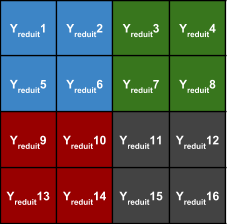
\includegraphics[scale=0.5]{images/yuv4.png}
\end{center}
\caption{Blocs réduits}
\label{}
\end{figure}

\bigbreak
Après avoir appliqué cette transformation sur l'ensemble de nos quatre blocs, on obtient quatre blocs aux dimensions variables en fonction de \texttt{zoiX} et \texttt{zoiY}.
Il y a cependant des agencements possibles de nos blocs qui donnent des dimensions constantes.
Après avoir réduit nos zones selon le principe que l'on vient de décrire, on leur trouve les dimensions suivantes :

\bigbreak
\begin{itemize}
\item{Zone 1 : \texttt{($\frac{\text{zoiX}}{2}$, $\frac{\text{imgHeight}}{2}$)}}
\item{Zone 2 : \texttt{($\frac{\text{imgWidth}-(\text{zoiX}+\text{zoiW})}{2}$, $\frac{\text{imgHeight}}{2}$)}}
\item{Zone 3 : \texttt{($\frac{\text{zoiW}}{2}$, $\frac{\text{zoiY}}{2}$)}}
\item{Zone 4 : \texttt{($\frac{\text{zoiW}}{2}$, $\frac{\text{imgHeight}-(\text{zoiY}+\text{zoiH})}{2}$)}}
\end{itemize}

\bigbreak
On peut tout de suite trouver un assemblage constant pour les zones 1 et 2 réduites : elles font la même hauteur et leur largeur commune ne dépend pas de la position de la ZOI : ils sont complémentaires.

$$ W_1 + W_2 = \frac{zoiX}{2} + \frac{imgWidth-(zoiX+zoiW)}{2} = \frac{imgWidth - zoiW}{2}$$
$$ = \mathbf{\frac{imgWidth}{4}} $$

\bigbreak
Les zones 1 et 2 l'une à côté de l'autre forment donc une zone de dimension constante \texttt{($\frac{imgWidth}{4}$, $\frac{imgHeight}{2}$)}.
Le même principe s'applique aux zones 3 et 4, avec cette fois-ci une largeur constante :

$$ H_3 + H_4 = \frac{zoiY}{2} + \frac{imgHeight-(zoiY+zoiH)}{2} = \frac{imgHeight - zoiH}{2} $$
$$ = \mathbf{\frac{imgHeight}{4}} $$

Les zones 3 et 4 l'une après l'autre forment donc une zone de dimension constante \texttt{($\frac{imgWidth}{4}$, $\frac{imgHeight}{4}$)}.
Nous avons choisi d'utiliser la répartition suivante :

\begin{figure}[H]
\begin{center}
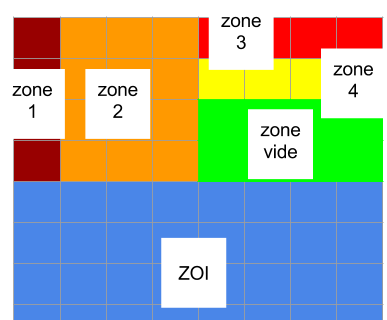
\includegraphics[scale=0.4]{images/decoupage2.png}
\end{center}
\caption{Organisation des zones}
\label{}
\end{figure}

\bigbreak
Nous obtenons ainsi une image d'une résolution de \texttt{640x720} pixels contenant notre ZOI inchangée et les autres zones sous-échantillonnées.
L'image après notre traitement ne pèse donc plus que la moitié de sa taille d'origine, avec un petit écart par rapport aux $\frac{7}{16}$ théoriques calculés.
Cet écart correspond à la zone verte sur notre schéma et ne véhicule aucune information vidéo.
Nous pourrions arranger différement les blocs en les découpant davantage mais nous avons fait le choix de conserver des blocs entiers pour éviter un calcul supplémentaire côté récepteur.

\subsection{Android}
Pour la partie réception mobile, nous avons choisi d'utiliser un smartphone Android comme support de développement.
En effet, le kit de développement offert par Google est gratuit, disponible sur des appareils mobiles et avec une puissance assez élevée pour effectuer du traitement vidéo en direct.
De plus, depuis quelques années, Google développe un écosystème de réalité de virtuelle pour Android.

\bigbreak
Nous avons donc développé une application Android en Java, qui récupère le flux video en Wi-Fi, décompresse la vidéo et l'affiche sur l'écran pour un casque de type Cardboard.
Cette application comporte une activité qui démarre la partie réception vidéo et affiche le flux vidéo. De plus, cette activité possède un menu qui permet à l'utilisateur d'activer ou non le traitement vidéo et de définir sa source vidéo (une une vidéo de test embarquée dans l'application ou le flux vidéo d'un émetteur).
Nous avons implémenté deux modules de réception vidéo différents mais qui implémente la même interface Java afin d'être facilement interchangeable par l'activité qui les lance.

\bigbreak
Le premier récepteur est une version simplifée qui utilise une vidéo stockée en local (dans l'application) afin de tester la partie traitement vidéo sans avoir à utiliser un émetteur.
Techniquement, c'est un thread qui va régulierement lire le flux vidéo et l'envoyer au décodeur vidéo. 
Pour lire le flux vidéo, nous utilisons un exctractor (class fournit par le SDK Android) qui permet de parser un fichier vidéo. Nous pouvons ensuite demander à l'extractor le type de vidéo contenue dans le fichier, puis d'écrire une partie partie du flux vidéo dans un buffer.
Pour décoder ce flux vidéo, nous utilisons l'API MediaCodec qui permet d'accéder au support multimédia bas-niveau fournit par le SDK. Ce MediaCodec permet, entre autres, de décoder un flux vidéo.
Pour fonctionner, nous configurons un mediaCodec avec les paramètres de la vidéo trouvés via l'extractor ainsi que la surface dans laquelle la vidéo décodée doit être envoyée (cette partie sera expliquée dans la sous-section suivante).
Puis, grâce à notre thread, nous allons régulièrement demander au mediaCodec de nous fournir un buffer, que nous transférons à l'extractor afin qu'il y ajoute les données suivantes du flux vidéo.
Le mediacodec recupère alors ce buffer, décode le flux vidéo qui y est présent et envoye les images décodées à la surface.
Ce mécanisme de réutilsiation des buffers, géré par MediaCodec, permet au développeur de ne pas avoir à s'occuper de l'allocation de gros volumes de données (qui pourrait être une source de perte de performance). 

\bigbreak
La deuxième implémentation du module de réception vidéo est similaire au précedant, hormis que l'on récupère le flux vidéo sur un équipement distant.
Ce module remplace donc l'extractor par deux sockets réseaux.
Tout d'abord, le récepteur se connecte à l'émetteur via une socket TCP pour initier le flux de contrôle.
Puis, il écoute sur un port UDP pour récuperer le flux vidéo.
Plus précisement, les datagrammes UDP contiennent des paquets MPEG-TS qui encapsule des fragments de paquets PES (Packetized Elementary Stream) qui correspondent aux données du flux vidéo.
Une fois un paquet PES reconstitué (à l'aide de plusieurs paquets MPEG-TS), il est transféré dans un buffer du mediaCodec afin que ce dernier décode ses données vidéos et les transmette à la surface.

\begin{figure}[H]
\begin{center}
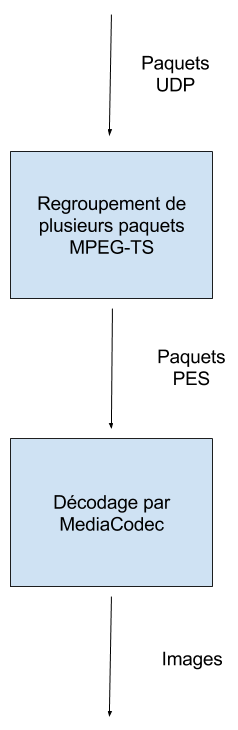
\includegraphics[scale=0.35]{images/decodage_video.png}
\end{center}
\caption{Schéma explicatif du décodage vidéo dans l'application Android}
\label{}
\end{figure}

\subsection{OpenGL ES}
Nous allons maintenant aborder la partie traitement vidéo effectuée au niveau du récepteur, c'est-à-dire translater les zones de l'image à leur place initiale et sur-échantillonner celles qui ont été sous-échantillonnées par l'émetteur.

\bigbreak
Pour rappel, ce traitement s'effectue après le décodage du flux vidéo, afin de pouvoir réutiliser un décodeur vidéo déjà existant.
Nous avions commencé par effectuer ce traitement en Java. 
Pour cela, nous récupérions l'image en sortie du décodeur, via un tableau de bytes, et nous parsions ses pixels et les recopions dans un autre tableau.
Cette partie de l'algorithme prennait trop de temps à s'exécuter pour un flux continu, c'est-à-dire que ce traitement était plus long que le délai inter-image du flux vidéo.
De plus, cette algorithme ne comportait que la partie translation et pas encore la partie sur-échantillonnage.

\bigbreak
C'est pourquoi, nous avons décidé d'effectuer ce traitement via OpenGL ES.
En effet, OpenGL ES (Open Graphics Library for Embedded System) est une API qui permet d'effectuer des calculs d'images. 
OpenGL ES est une simplification de OpenGL optimisée pour les appareils mobiles et est bien intégrée dans Android.
C'est la façon la plus courante d'utiliser la puce graphique d'un appareil depuis une application Android.

\bigbreak
Pour pouvoir utiliser OpenGL ES dans notre application, nous avons intégré une surfaceTexture dans notre activité.
Une surfaceTexture est un objet qui nous permet d'effectuer un traitement OpenGL ES sur un flux vidéo.
Contretement, la surfaceTexture récupère un flux vidéo en entée, appelle une fonction de call-back à chaque nouvelle image, et renvoie le flux en direct à une surface.
Une surface encapsule un tableau d'une image raw qui est envoyé au controleur vidéo du mobile afin d'être affiché l'image sur l'écran de l'appareil.
Il nous suffit donc d'effectuer nos appels OpenGL ES dans la fonction de call-back proposée par la surfaceTexture.

\bigbreak
Comme expliqué dans la partie émetteur, le récepteur reçoit un flux vidéo traité dont les zones de l'image sont translatées et certaines sous-échantillonnées.
De plus, le récepteur connait la position initiale du point haut gauche de la ZOI (via la connexion TCP).
Connaissant les résolutions initiniales et finales de toutes les zonez, le récepteur peut en déduire les coordonnées des zones dans l'image reçue et dans l'image à afficher.

\begin{figure}[H]
\begin{center}
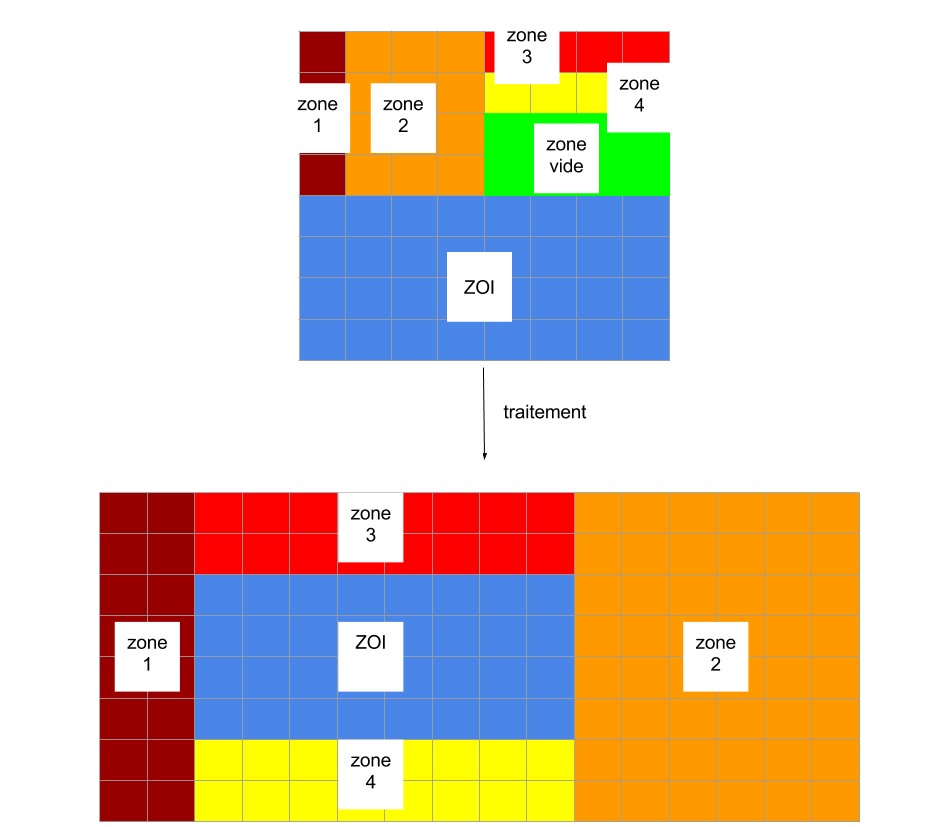
\includegraphics[scale=0.35]{images/schema_traitement_video_retour.png}
\end{center}
\caption{Schéma explicatif du traitement vidéo effectué par OpenGL ES}
\label{}
\end{figure}

\bigbreak
Ce traitement est assez simple à programmer pour OpenGL ES, il suffit de connaitre les coordonnées avant et après traitement pour tous les blocs.
De plus, si l'aire après traitement d'un bloc est plus grande que l'aire initiale, alors OpenGL ES effectuera automatiquement un sur-échantillonnage.
La seule subtilitée à savoir est que, pour de la 2D, OpenGL ES ne sait pas utiliser des rectangles mais uniquement des triangles.
Il faut donc utliser deux triangles par bloc afin de les traiter entierement.
Ainsi, si l'on veut transformer un bloc de coordonnnées ABCD en un bloc de coordonnées EFGH, il suffit d'envoyer trois listes à OpenGL ES :

\bigbreak
\begin{itemize}
\item{[A, B, C, D] : coordoonées de départ}
\item{[E, F, G, H] : coordoonées d'arrivée}
\item{[0, 1, 2, 0, 2, 3] : positions, dans les listes précédantes, des coordonnées des triangles à copier dans la surface finale (ABC => EFG et ACD => EGH)}
\end{itemize}

\begin{figure}[H]
\begin{center}
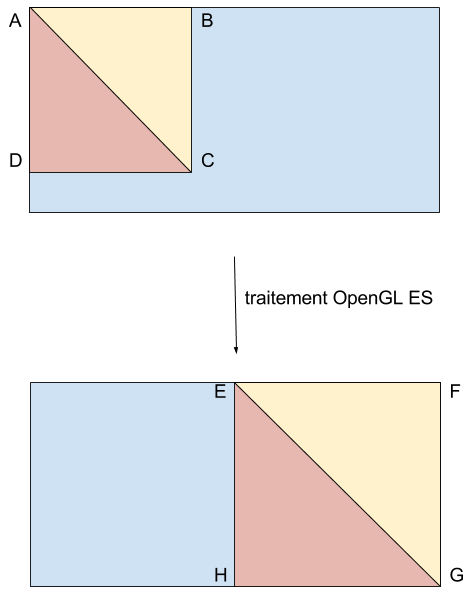
\includegraphics[scale=0.35]{images/OpenGL_ES.png}
\end{center}
\caption{Example de traitement sur un bloc via OpenGL ES}
\label{}
\end{figure}

\subsection{Cardboard}
Pour terminer la partie sur le récepteur Android, nous allons maintenant aborder la partie réalité virtuelle avec le Cardboard.
En effet, une des raisons principales qui a motivé notre choix vers Android comme base du récepteur, est le SDK Cardboard qui fonctionne lorsque le téléphone est placé dans un casque de réalité virtuelle compatible.
Ainsi, l'application Anroid peut demander au SDK l'angle de vision de l'utilisateur à tout instant, le SDK va scinder l'écran en deux, appeler une fonction de call-back à chaque fois qu'il va dessiner l'image pour un des deux yeux, et appliquer un filtre pour corriger la distortion que rend les lentilles placées dans le casque.


\bigbreak
De plus, le SDK nous permet d'avoir une fonction de call-back qui sera appelée à chaque que l'image est dessinée pour un oeil.
Dans cette fonction nous effectuons un dexuieme traitement OpenGL ES afin de déplacer l'image en fonction de l'angle de vision de l'utilisateur (récupéré via le SDK Cardboard) et nous zommons x2 dans l'image afin que l'utilisateur voit uniquement la zone correspondant à l'endroit où il regarde à un instant donné.
Pour effectuer ce traitement, nous utilisons une matrice et les fonctions annexes que propose OpenGL ES.
Tout d'abord nous créons une matrice identitaire, que nous translatons (via une fonction dédiée) vers le haut gauche de la zone que souhaite voir l'utilisateur, puis nous 


\section{Résultats}

\section{Conclusion}

\end{document}
